%%%%%%%%%%%%%%%%%%%%%%%%%%%%%%%%%%%%%%%%%%%%%%%%%%%%%%%%%%%%%%%%%%%%%%%%%%%

\documentclass{standalone}

\usepackage{mathptmx}
\usepackage{tikz}
\usetikzlibrary{angles}
\usetikzlibrary{external}
\usetikzlibrary{quotes}
\tikzexternalize{unit-circle-right-triangle}

%% We default to Times.
\renewcommand{\rmdefault}{ptm}
\renewcommand{\ttdefault}{pcr}
%% Enable Times/Palatino main text font.
\normalfont\selectfont

\newcommand{\comma}{,\,}
\newcommand{\tuple}[2]{(#1\comma #2)}

%% A generic point on the unit circle.
\newcommand{\genericPoint}{%%
  %% The generic point.
  \xyPoint{\xa}{\yb}{\tuple{a}{b}}{above right}
  %% The origin.
  \xyPoint{0}{0}{\tuple{0}{0}}{left}
  %% The third point.
  \xyPoint{\xa}{0}{\tuple{a}{0}}{right}
  %% Label the angle.
  \path pic["$\varphi$",draw,->,thick,angle radius=1cm] {angle=xyRadius--origin--point};
  %% The right-triangle.
  \draw[lineStyle] (origin) -- (point) -- (\xa,0) -- cycle;
  %% A vertical line meets at the generic point.
  \node at (\xa,\yb/2) [right] {$b$};
  %% A horizontal line meets at the generic point.
  \node at (\xa/2,0) [below] {$a$};
}

%% A point on the Cartesian plane.
%%
%% #1 -- The x-coordinate of the point.
%% #2 -- The y-coordinate of the point.
%% #3 -- Label the point with this name.
%% #4 -- Where to place the label relative to the point.
\newcommand{\xyPoint}[4]{%%
  \node[nodeStyle] at (#1,#2) {};
  \node at (#1,#2) [#4] {$#3$};
}

%%%%%%%%%%%%%%%%%%%%%%%%%%%%%%%%%%%%%%%%%%%%%%%%%%%%%%%%%%%%%%%%%%%%%%%%%%%
%% Generic values of sine and cosine in the unit circle.
%%%%%%%%%%%%%%%%%%%%%%%%%%%%%%%%%%%%%%%%%%%%%%%%%%%%%%%%%%%%%%%%%%%%%%%%%%%

\begin{document}

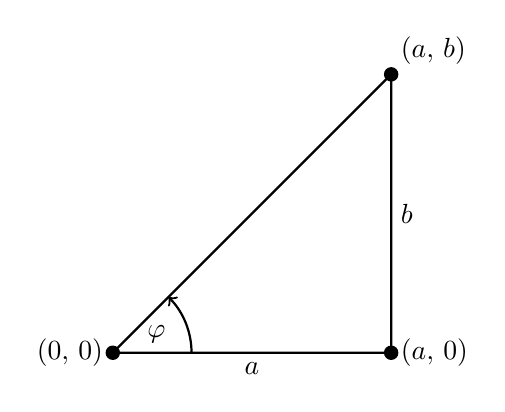
\begin{tikzpicture}[%%
  lineStyle/.style={-,thick},%%
  nodeStyle/.style={draw,inner sep=1.7pt,circle,fill=black,black}%%
]
%%
%%
\pgfmathsetmacro{\radius}{5}
\pgfmathsetmacro{\xa}{3.53553390593274}  %% A point at 45 degrees.
\pgfmathsetmacro{\yb}{\xa}
%% The Cartesian coordinate system.
\coordinate (origin) at (0,0);
%% The generic angle.
\coordinate (point) at (\xa,\yb);
\coordinate (xyRadius) at (\radius,0);
%%
%%
%% Illustrate a generic right-triangle within a unit circle.
\genericPoint
\end{tikzpicture}

\end{document}
